\documentclass{standalone}
\usepackage{tikz}
\usetikzlibrary{shapes.geometric, arrows}

\definecolor{mycolor}{RGB}{0, 153, 255}
\tikzstyle{process} = [rectangle, rounded corners,
                       minimum width=2cm, minimum height=1cm,
                       text centered, draw=black, fill=mycolor,
                       text=white, line width=0.3mm]

\tikzstyle{arrow} = [thick,->,>=stealth]

\begin{document}
    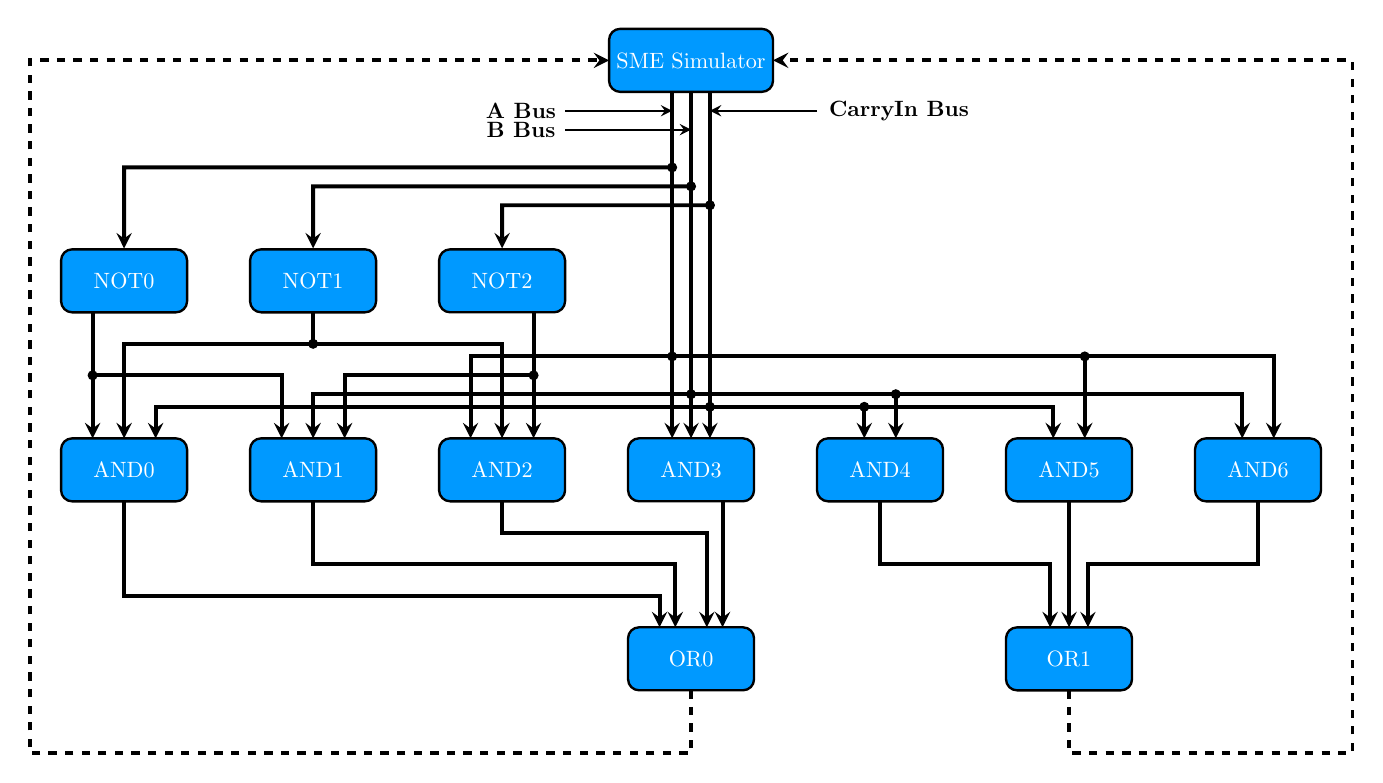
\begin{tikzpicture}[node distance=2cm, scale=0.8, every node/.style={scale=0.8}]
        
        \node at (0,1)(Simulator) [process] {SME Simulator};
        \draw [arrow] (-2, 0.2) -- (-0.3,0.2);
        \node at (-2.7,0.2) {\textbf{A Bus}};
        \draw [arrow] (-2, -0.1) -- (0,-0.1);
        \node at (-2.7,-0.1) {\textbf{B Bus}};
        \draw [arrow] (2, 0.2) -- (0.3,0.2);
        \node at (3.3,0.2) {\textbf{CarryIn Bus}};
        
        %NOT Gates
        \node (NOTC) [process, below of = Simulator, xshift=-3cm, yshift=-1.5cm] {NOT2};
        \node (NOTB) [process, left of = NOTC, xshift=-1cm, yshift=0cm] {NOT1};
        \node (NOTA) [process, left of = NOTB, xshift=-1cm, yshift=0cm] {NOT0};
        
        %Simulator to NOT gates
        \draw [arrow, line width=0.5mm] (-0.3, -0.7) -- (-9,-0.7) --  (NOTA);
        \filldraw[black] (-0.3, -0.7) circle (2pt);
        \draw [arrow, line width=0.5mm] (-0, -1) -- (-6,-1) --  (NOTB);
        \filldraw[black] (-0, -1) circle (2pt);
        \draw [arrow, line width=0.5mm] (0.3, -1.3) -- (-3,-1.3) --  (NOTC);
        \filldraw[black] (0.3, -1.3) circle (2pt);
        
        %AND Gates
        \node (AND3) [process, below of = NOTC, xshift=3cm, yshift=-1cm] {AND3};
        \node (AND2) [process, left of = AND3, xshift=-1cm] {AND2};
        \node (AND1) [process, left of = AND2, xshift=-1cm] {AND1};
        \node (AND0) [process, left of = AND1, xshift=-1cm] {AND0};
        
        \node (AND4) [process, right of = AND3, xshift=1cm] {AND4};
        \node (AND5) [process, right of = AND4, xshift=1cm] {AND5};
        \node (AND6) [process, right of = AND5, xshift=1cm] {AND6};
                
        %Lines to AND0 gate
        \draw [arrow, line width=0.5mm] (-9.5, -3) --   (-9.5, -5);
        \draw [arrow, line width=0.5mm] (0.3, -4.5) -- (-8.5,-4.5) -- (-8.5,-5);
        \filldraw[black] (0.3, -4.5) circle (2pt);
        \draw [arrow, line width=0.5mm] (-6, -3) -- (-6,-3.5) -- (-9,-3.5) -- (-9,-5);
        \filldraw[black] (-6,-3.5) circle (2pt);
        
        %Lines to AND1 gate
        \draw [arrow, line width=0.5mm] (-9.5, -4) --  (-6.5, -4) -- (-6.5, -5);
        \filldraw[black] (-9.5, -4) circle (2pt);
        \draw [arrow, line width=0.5mm] (-2.5,-4) -- (-5.5,-4) -- (-5.5,-5);
        \filldraw[black] (-2.5,-4) circle (2pt);
        \draw [arrow, line width=0.5mm] (0,-4.3) -- (-6,-4.3) -- (-6,-5);
        \filldraw[black] (0,-4.3) circle (2pt);
        
        %Lines to AND2 gate
        \draw [arrow, line width=0.5mm] (-2.5, -3) --  (-2.5, -5);
        \draw [arrow, line width=0.5mm] (-6, -3) -- (-6,-3.5) -- (-3,-3.5) -- (-3,-5);
        \draw [arrow, line width=0.5mm] (-0.3, -3.7) -- (-3.5,-3.7) -- (-3.5,-5);
        \filldraw[black] (-0.3, -3.7) circle (2pt);
        
        %Lines to AND3 gate
        \draw [arrow, line width=0.5mm] (0,0.5) -- (0, -5);
        \draw [arrow, line width=0.5mm] (0.3,0.5) --  (0.3, -5);
        \draw [arrow, line width=0.5mm] (-0.3,0.5) --  (-0.3, -5);
        
        %Lines to AND4 gate
        \draw [arrow, line width=0.5mm] (0.3,-4.5) -- (2.75, -4.5) -- (2.75, -5);
        \draw [arrow, line width=0.5mm] (0,-4.3) -- (3.25, -4.3) -- (3.25, -5);
        
        %Lines to AND5 gate
        \draw [arrow, line width=0.5mm] (0.3,-4.5) -- (5.75, -4.5) -- (5.75, -5);
        \filldraw[black] (2.75, -4.5) circle (2pt);
        \draw [arrow, line width=0.5mm] (-0.3,-3.7) -- (6.25, -3.7) -- (6.25, -5);
        
        %Lines to AND6 gate
        \draw [arrow, line width=0.5mm] (-0.3,-3.7) -- (9.25, -3.7) -- (9.25, -5);
        \filldraw[black] (6.25, -3.7) circle (2pt);
        \draw [arrow, line width=0.5mm] (0,-4.3) -- (8.75, -4.3) -- (8.75, -5);
        \filldraw[black] (3.25, -4.3) circle (2pt);
        
        %OR gates
        \node (OR0) [process, below of = AND3, xshift=-0cm, yshift=-1cm] {OR0};
        \node (OR1) [process, right of = OR0, xshift=4cm, yshift=-0cm] {OR1};
        
        %Lines to OR0 gate
        \draw [arrow, line width=0.5mm] (0.5,-6) -- (0.5, -8);
        \draw [arrow, line width=0.5mm] (-3,-6) -- (-3, -6.5) -- (0.25, -6.5) -- (0.25, -8);
        \draw [arrow, line width=0.5mm] (-6,-6) -- (-6, -7) -- (-0.25, -7) -- (-0.25, -8);
        \draw [arrow, line width=0.5mm] (-9,-6) -- (-9, -7.5) -- (-0.5, -7.5) -- (-0.5, -8);
        
        %Lines to OR1 gate
        \draw [arrow, line width=0.5mm] (6,-6) -- (6, -8);
        \draw [arrow, line width=0.5mm] (3,-6) -- (3, -7) -- (5.7,-7) -- (5.7, -8);
        \draw [arrow, line width=0.5mm] (9,-6) -- (9, -7) -- (6.3,-7) -- (6.3, -8);
                
        %Output lines to simulator
        %OR1 output
        \draw [arrow, line width=0.5mm, dashed] (0,-9) -- ++(0, -1) -- ++(-10.5,0) -- ++(0,11) -- ++(9.2,0);
        \draw [arrow, line width=0.5mm, dashed] (6,-9) -- ++(0, -1) -- ++(4.5,0) -- ++(0,11) -- ++(-9.2,0);
    
    \end{tikzpicture}
\end{document}
